\section{Introduction}

\begin{figure}[t]
    \centering
    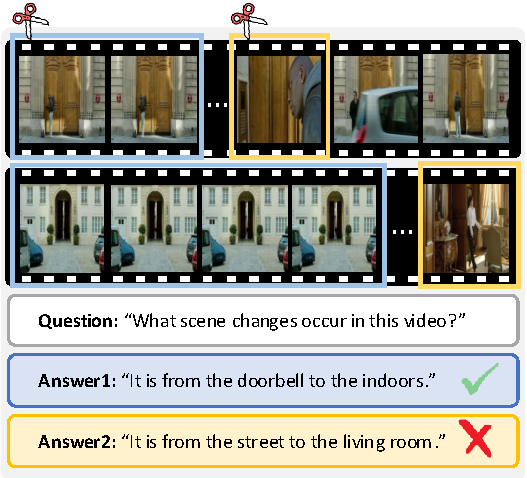
\includegraphics[width=\linewidth]{latex/figures/intro.pdf}
    \vspace{-7mm}
    \caption{\textbf{Power of frame uniqueness.} Removing \textcolor[RGB]{56,94,181}{\textbf{24} redundant frames} results in \textcolor[RGB]{29,195,136}{\textbf{accurate}} video understanding by VideoLLMs, while dropping just \textcolor[RGB]{248,170,52}{\textbf{8} unique frames} leads to \textcolor[RGB]{223,52,39}{\textbf{inaccurate}} video comprehension, highlighting the critical role of unique frames for VideoLLMs.}
    \vspace{-5mm}
    \label{fig:motivation}
\end{figure}



Recently, Video Large Language Models (VideoLLMs) have demonstrated remarkable performance in video understanding and reasoning tasks~\cite{Zhang:Video-LLaMA,wang2025internvideo2.5}. However, videos inherently contain multiple consecutive frames, resulting in a significantly higher number of visual tokens compared to images. For instance, LLaVA-OneVision~\cite{li2024llava-ov} processes $32 \times 196$ visual tokens per video, while LLaVA-Video~\cite{zhang2024llava-video} handles even more at $64 \times 182$ visual tokens. This high token count inevitably leads to expensive computation~\cite{liu2025shifting}, especially for long video understanding~\cite{chen2024longvila}.



To mitigate this computational burden, researchers have turned to token compression methods~\cite{Chen:FastV,Yang2024:Visionzip}, considering the inherent visual redundancy and aiming to minimize redundant visual information. 
These approaches can be categorized as pre-LLM~\cite{Zhang:FasterVLM} or intra-LLM~\cite{Chen:FastV} methods, based on whether compression occurs before or within the LLM.
Most of these methods are training-free, enabling plug-and-play inference acceleration for existing VideoLLMs. 
However, despite these efforts, existing token compression methods suffer from \textbf{\emph{two critical issues}}: 

% \paragraph{(I) Design Myopia}
\noindent \textbf{(I) Design Myopia:} In human video perception, we naturally focus on distinctive frames (\textit{e.g.}, those with significant spatio-temporal changes) while ignoring repetitive and redundant visual information~\cite{ma2025mmg-vid}. By contrast, most existing token compression methods apply a \textit{uniform} compression strategy across all frames, treating each one as equally informative. Even recent VideoLLM-specific method DyCoke~\cite{tao2024dycoke} exhibits this limitation by grouping every four consecutive frames into a fixed window and compressing them identically, without regard for the varying distinctiveness of individual frames. Figure~\ref{fig:motivation} further illustrates the critical nature of this issue: removing 24 redundant frames does not affect the accurate response of the LLaVA-OneVision, whereas dropping just 8 unique frames causes it to fail, despite being only a \textbf{third} of the number. This contrast shows that uniform compression risks discarding critical information in unique frames that VideoLLMs may rely on, thereby significantly impacting overall performance. Notably, Table~\ref{tab:main_results} indicates that some methods even \textbf{underperform} random token dropping, further indicating their sub-optimal performance.



\begin{table}[!t]
  \centering
  \setlength{\tabcolsep}{0.4pt} % 调整列间距
    \scalebox{0.73}{\begin{tabular}{lcccccc}
    \multirow{2}{*}{\textbf{Methods}} & \textbf{Pre-} & \textbf{Intra-} & \textbf{\texttt{[CLS]}} & \textbf{Video-} & \textbf{Frame} & \textbf{Efficient} \\
    
    & \textbf{LLM} & \textbf{LLM} & \textbf{Dependency} & \textbf{Specific} & \textbf{Uniqueness} & \textbf{Attention} \\
    \shline
     FastV &  & \cmark &  &  &  &  \\
     PDrop &  & \cmark &  &  &  &  \\
     SparseVLM &  & \cmark &  &  &  & \\
     MUSTDrop & \cmark & \cmark & \cmark &  &  &  \\
     FiCoCo & \cmark & \cmark & \cmark &  &  &  \\
     FasterVLM & \cmark &  & \cmark &  &  & \cmark \\
     DyCoke & \cmark &  &  & \cmark &   & \cmark \\
    \rowcolor[rgb]{ .949,  .949,  .949}
    \textbf{VidCom$^2$} & \cmark &  &  & \cmark &  \cmark & \cmark \\
    \end{tabular}%
    }
    \vspace{-2mm}
  \caption{\textbf{Feature comparison with existing training-free token compression methods.} Most suffer from design myopia and implementation constraints.}
  \label{tab:para_comparsion}%
  \vspace{-5mm}
\end{table}%


% \paragraph{(II) Implementation Constraints}
\noindent \textbf{(II) Implementation Constraints:} 
Beyond design limitations, existing methods face practical constraints. Some token compression works~\cite{Zhang:FasterVLM,Liu2024:MUSTDrop} rely on \texttt{[CLS]} attention weights in ViT for informative token preservation, yet modern VideoLLMs adopt SigLIP~\cite{ZhaiM0B23:SigLIP} as visual encoder without \texttt{[CLS]} token. Meanwhile, certain methods~\cite{Zhang:SparseVLM,xing2024pdrop} aim to leverage textual information but require explicit attention weights in specific LLM layers, making them incompatible with efficient attention operators~\cite{Dao2022:FlashAttention}. This incompatibility leads to higher peak memory usage, even \textbf{surpassing} that of uncompressed processing (see Table~\ref{tab:efficiency_comparisons}), which is especially problematic for long video understanding~\cite{wen2025token,wen2025dart}.


We summarize existing works in Table~\ref{tab:para_comparsion} and identify \textbf{\emph{three key principles}} for designing effective and efficient token compression methods for VideoLLM:
\textbf{(i) Model Adaptability:} The method should be easily compatible with and adaptable to the majority of existing VideoLLMs~\cite{zhang2024llava-video,Wang:Qwen2-VL}; \textbf{(ii) Frame Uniqueness:} The method should consider varying distinctiveness across video frames;
\textbf{(iii) Operator Compatibility:} The method should maintain compatibility with efficient operators~\cite{daoFlashAttention-2}.


Based on above analysis, we propose ``\textbf{Vid}eo \textbf{Com}pression \textbf{Com}mander'' (\textit{i.e.}, \textbf{VidCom$^2$}), an efficient plug-and-play token compression method for VideoLLMs from the perspective of frame uniqueness. Our VidCom$^2$ follows a principled two-stage approach: first adjusting frame-wise compression intensity based on each frame's uniqueness in the video sequence, then performing token compression by evaluating token distinctiveness both within individual frames and across the entire video. Through this careful design, VidCom$^2$ mimics human video perception by adaptively adjusting attention to different frames (see Figure~\ref{fig:frame_uniqueness_vidcom2}), preserving information from key frames while minimizing redundant visual content.


In summary, our contributions are three-fold:
\begin{itemize}

    \item \textbf{Empirical Method Analysis:} We critically analyze existing token compression methods, unveiling their inherent limitations and delineating three key design principles for effective and efficient VideoLLM token compression.
    
    \item \textbf{Video Compression Commander:} We are the first to propose a VideoLLM token compression framework based on frame uniqueness, offering a plug-and-play method with frame-wise dynamic compression.
    
    \item \textbf{Outstanding Performance \& Efficiency:} Extensive experiments on diverse benchmarks demonstrate superior efficiency-performance trade-offs. With 15\% tokens, VidCom$^2$ outperforms the second-best method by \textbf{3.9\%} and \textbf{2.2\%} on LLaVA-OV and LLaVA-Video.

    
\end{itemize}
